\documentclass{scrartcl}

%\usepackage{etex}
\usepackage[left=3cm,right=2.0cm,top=1.25cm,bottom=1.75cm,includehead,includefoot]
{geometry}
\usepackage{marginnote}
\reversemarginpar
%Math
\usepackage{amsfonts,amsmath,amssymb,amsthm, amstext}
%Language, encoding, ...
\usepackage[utf8]{inputenc}
\usepackage[T1]{fontenc}
\usepackage[english]{babel}
\usepackage{t1enc, lmodern, textcomp}
%Pictures
\usepackage{graphicx, color}
%\usepackage{latexsym}
%\usepackage{keyval}
%\usepackage{ifthen}
%\usepackage{moreverb}
\usepackage[shell]{gnuplottex}
%Colors
\usepackage[usenames,dvipsnames]{xcolor}
\definecolor{darkblue}{rgb}{0.0, 0.2, 0.6}
\renewcommand*{\marginfont}{\bf\color{darkblue}}
%Nice a/b fractions
\usepackage{xfrac}
%Make it possible to write (fat) upright greek letters
\usepackage{upgreek}

%For indices
\newcommand{\ix}[1]{_{\mathrm{#1}}}
\newcommand{\Ix}[1]{^{\mathrm{#1}}}

%Directly include svg images
%%%%%%%%%%%%%%%%%%%%%%%%%%%%%%%%%%%%%%%%%%%%%%%%%%
\newcommand{\executeiffilenewer}[3]{%
    \ifnum\pdfstrcmp{\pdffilemoddate{#1}}%
    {\pdffilemoddate{#2}}>0%
    {\immediate\write18{#3}}\fi%
}
\newcommand{\includesvg}[1]{%
    \executeiffilenewer{#1.svg}{#1.pdf}%
    {inkscape -z -D --file=#1.svg %
    --export-pdf=#1.pdf --export-latex}%
    \input{#1.pdf_tex}%
}
%%%%%%%%%%%%%%%%%%%%%%%%%%%%%%%%%%%%%%%%%%%%%%%%%%

%Make captions look okay
\usepackage[font=small,format=plain,labelfont=bf,up,up]{caption}

%Hyperlinks
\usepackage{hyperref}
\hypersetup{
            pdflang=en-EN,
            unicode=true,
            pdfauthor={Thomas Staudt, Erik Schultheis},
}

%Differential d's
\newcommand{\dif}{\mathrm{d}}
\newcommand{\tdif}[2]{\ensuremath{\frac{\dif#1}{\dif#2}}}
\newcommand{\pdif}[2]{\ensuremath{\frac{\partial#1}{\partial#2}}}
\newcommand{\ppdif}[2]{\ensuremath{\frac{\partial^{2}#1}{\partial#2^{2}}}}
%Degree
\newcommand{\degr}{^\circ}

\renewcommand{\refname} {Literature}
\renewcommand{\figurename}{\bf Figure}
\newcommand{\fs}[1]{\footnotesize #1}
%double slash
\newcommand{\git}{\mathbin{
  \mathchoice{\textbackslash\mkern-6mu\textbackslash}% \displaystyle
    {\textbackslash\mkern-6mu\textbackslash}% \textstyle
    {\textbackslash\mkern-5mu\textbackslash}% \scriptstyle
    {\textbackslash\mkern-5mu\textbackslash}}}% \scriptscriptstyle


%Bibliography
\usepackage[babel]{csquotes}
\usepackage[backend=bibtex8]{biblatex}


\newcommand*{\defeq}{\mathrel{\vcenter{\baselineskip0.5ex \lineskiplimit0pt
                     \hbox{\scriptsize.}\hbox{\scriptsize.}}}%
                     =}



%\bibliography{sources}


\begin{document}

\begin{titlepage}\centering
\textsc{\Large Institute For Nonlinear Dynamics \\[1.5ex] Universität Göttingen}

\vspace*{2cm}
{\huge A Practical Course On Network Science}
\vspace*{2cm}

\rule{\textwidth}{1pt}\\[0.5cm]
{\bfseries \huge Block A: \\[0.5cm] \huge \bfseries Random Networks\\[0.5cm]}
\rule{\textwidth}{1pt}

\vspace*{4cm}

\begin{Large}\begin{tabular}{rl}
        \textbf{Participants:}  & Erik Schultheis                                \\    
                   & \textit{erik.schultheis@stud.uni-goettingen.de}\\[0.5cm]
                   & Thomas Staudt                                  \\
                   & \textit{thomas.staudt@stud.uni-goettingen.de}  \\[1.0cm]

       \textbf{Tutors:}        & Dr. Nora Molkenthin, Benjamin Schäfer, Malte Schröder  \\[1.0cm]
       \textbf{Deadline:}      & 19.05.2015
\end{tabular}\end{Large}

\vspace*{1.5cm}

%\begin{Large}
%\fbox{
  %\begin{minipage}[t][2.5cm][t]{6cm} 
      %Attestation:
  %\end{minipage}
%}
%\end{Large} 

\end{titlepage}

\tableofcontents
\clearpage

\section{Random Networks}
\subsection{Erdös-Rényi Networks}
An Erdös-Rényi is a network generated by starting from a set of vertices $V$ in which for each possible edge $(v1, v2) \in V^2$ is present with probability $p$. This means that the runtime of a naive implementation of this generator is of order $O(|V|^2)$. An alternative is to start from the known degree distribution of any vertex 
\begin{align}
p(k) = \left( \begin{array}{c}n-1 \\ k \end{array} \right) p^k (1-p)^{n-1-k} \label{eq:degree_hist}
\end{align}, from which we get the distribution of total edge number by summing over all $n$ vertices (counting twice). 
Since we know that all edges are equally probable, we now can first determine the total number of edges present according to $P$, and then select the appropriate amount of edges randomly, decreasing the running time by a factor of $p$.

The results of this algorithm can be seen in fig. \ref{11_er}, where we have used a preselected number of edges instead of an edge probability to generate the graphs.
The degree distribution eq. \eqref{eq:degree_hist} is vizualized in figure \ref{fig:12_er}.

\subsection{Watts-Strogatz Networks and Small World Effect}
Many real world networks exhibit so called \emph{small world behaviour}, i.e. most connections are local (high clustering coefficient) but there are sufficently many global shortcuts to yield small average path length. This cannot be achieved with (sparse) Erdös-Rényi networks, however, the description above already gives us a starting point for a new graph generator algorithm, called Watts-Strogatz algorithm: Start with a graph that only has local connections (in the original version a ring with $k$ connections per node), and then rewire each edge with probability $p$ to a long range connection. This can be seen in figure \ref{13_ws}.

To find out when a Watts-Strogatz graph fulfills the small world condition, we look at average path length $L$ and clustering coefficient $C$ in dependence of $p$. For $k=2$, there is almost no clustering because the initial regular ring does not contain any triangles. Therefore, we look at $k=4$ (fig. \ref{13_ws} b) We see in fig. \ref{fig:13_sm_effect} that there is a region in which average path length is already low while local clustering is still high. Therefore, the Watts-Strogatz algorithm is well suited for generating small world networks.

We would like to make an analgue investigation for Erdös-Rényi graphs. However, we cannot directly compare the behaviour of Erdös-Rényi and Watts-Strogatz networks with respect to $p$, because the parameter describes two totally different things in those models: For Erdös-Rényi, the number of edges depends on $p$. In particular, $p=0$ implies an edgefree graph, so the average path length is undefined. 

Nonetheless, we can plot $L$ and $C$ over the edge probability $p$, to find if there is a parameter region for which Erdös-Rényi produces a small world graph. Is evident in figure \ref{fig:13_sm_effect} b) this only happens when $p$ approaches $1$, i.e. when the graph is no longer sparse.

\subsection{Watts-Strogatz on a Regular Grid}
Finally, we investigate the Watts Strogatz algorithm applied to regular grid instead of a ring topology. We limited our investigation to square lattices with a manhatten metric. We chose the parameter $k$ to denote the maximum length of the initial connections, i.e. every grid node is connected to every other node within a circle of radius $k$. Such a grid is visualized in fig. \ref{fig:15_sm_2d} b). 

Due to its two dimensional nature, the grid offers, even without rewiring, relatively short path lengths and high clustering, because distances only grow with $\sqrt{N}$ as opposed to $N$ in the ring topology. This can be seen in figure \ref{fig:15_sm_2d} a): We see only a slight reduction in average path length as $p$ increases, because we already start with a low values. If our initial grid had been larger, this difference would be more significant. We can estimate the minimum possible average path length as follows:
Let each node be, on average, connected to $K$ nodes. Then we can reach $K^l$ nodes after $l$ steps, for the average path length to all other nodes we have $K^l \sim N$ and thus $l \sim \log N$. Therefore, we expect this behaviour for $p \rightarrow 1$, so the path length will fall from $\sqrt{N}$ to $\log N$, which will be much more noticable for larger grids. We chose $N=484$ in figure to make the data comparable to the other graphs in figure \ref{fig:13_sm_effect}. 

\begin{figure}
    \centering
    \def\svgwidth{0.8\columnwidth}
    \input{pictures/11_er_lat.pdf_tex}
    \marginnote{A.1.1}
    \caption{Visualization of Erdös-Renyi networks with $n=20$ nodes and $10$ (figure \textbf{a)}) as well as $20$ (figure \textbf{b)})
        edges. Thus the fraction of existent edges are $p \approx 0.0526$
        respectively $p \approx 0.1053$. The colors of the edges indicate the time
        steps at which it was added.}
    \label{11_er}
\end{figure}

\begin{figure}
    \centering
    \def\svgwidth{0.8\columnwidth}
    \input{pictures/13_ws_lat.pdf_tex}
    \marginnote{A.1.3}
    \caption{Visualization of Watts-Strogatz networks with two different
        sets of parameters. In figure \textbf{a)} $n=10$, $k=2$, and
        $p=0.4$, and in figure \textbf{b)} $n=16$, $k=4$, and $p=0.2$. In
        both figures, the reconnected edges are colored red. For figure
        \textbf{a)} the additional dashed lines mark the original graph
    before rewiring (i.e.\ the network for $p=0$).}
    \label{13_ws}
\end{figure}

\begin{figure}
    \gnuplotloadfile[terminal=epslatex, terminaloptions={color size 6.5,2.0}]{pictures/12_er_hist.gp}
    \marginnote{A.1.2}
    \caption{Degree distribution of Erdös-Renyi networks for \textbf{a)}
    fixed $n=350$ and varying values of $p$ and \textbf{b)} varying values
    of $n$ and fixed $p=0.1$. For figure \textbf{b)} the degree value $k$ was
    divided by the value $p(N-1)$ for which the degree distribution $P$
    (theoretically) takes its maximum, so that the different shapes of the
    distributions are highlighted.}
    \label{fig:12_er}
\end{figure}

\begin{figure}
    \centering
    \gnuplotloadfile[terminal=epslatex, terminaloptions={color size 5,2.0}]{pictures/12_largest.gp}
    \marginnote{A.1.2}
    \caption{The size of the largest cluster for Erdös-Renyi networks of
        size 500 in dependence of the parameter $p$. In order to obtain the
        values, 500 trials were done for every point of data.}
    \label{fig:12_largest}
\end{figure}


\begin{figure}
    \gnuplotloadfile[terminal=epslatex, terminaloptions={color size 6.5,2.0}]{pictures/13_sm.gp}
    \marginnote{A.1.2 A.1.4}
    \caption{Comparison of the small-world effect for \textbf{a)}
    Watts-Strogatz networks and \textbf{b)} Erdös-Renyi networks. In both
    cases the average path length $L$ and the clustering coefficient $C$
    were given as function of the parameter $p$ of the respective model.
    Note that $p_\mathrm{r}$ in the Watts-Strogatz model denotes the
    \emph{rewire probability} and has nothing to do with the
    \emph{occupation probability} $p_\mathrm{o}$ (which is also the reason
    for the different notations here). For better comparability all values
    of $L$ and $C$ were normed with the initial values ($p_r=0$) of the
    Watts-Strogatz network.}
    \label{fig:13_sm_effect}
\end{figure}

\begin{figure}
    %\gnuplotloadfile[terminal=epslatex, terminaloptions={color size 6.5,2.0}]{pictures/15_2d.gp}
    \input{pictures/15_2d_full.pdf_tex}
    \marginnote{A.1.5}
    \caption{Figure \textbf{a)}: The small world effect for the
        Watts-Strogatz algorithm in two dimensions. A $22\times22$ grid was used with $k=3$
        for a simulation over 10 trials (analogous to the simulations
        conducted for figure \ref{fig:13_sm_effect}). For reasons of
        comparison, both $L$ and $C$ were divided by the same initial values
        $L_\mathrm{WS}(0)$ and
        $C_\mathrm{WS}(0)$ that were also used in figure
        \ref{fig:13_sm_effect}. Figure \textbf{b)}: Visualization of the
        Watts-Strogatz algorithm in a 2d grid of size $5\times 5$ with $k = 1$ and $p = 0.2$. The
        dashed lines are existent edges before the algorithm is applied. After it is
        applied, the dashed lines become the red ones instead.}
    \label{fig:15_sm_2d}
\end{figure}

\clearpage
\section{Scale-Free Networks and Robustness}
\subsection{Barab\'asi-Albert Networks}
Real networks often exhibit the so called \emph{scale-free property},
meaning that their degree distribution $P_\mathrm{d}(k)$, which is the probability
that a randomly selected node has degree $k$, follows a power law
\begin{equation}
    P_\mathrm{d}(k) \sim k^{-\gamma}
\end{equation}
with the \emph{scaling exponent} $\gamma$. One usually has $2 \le \gamma \le 4$.

In 1991, Barab\'asi and Albert proposed an algorithm that generates
scale-free networks, which is based on \emph{growth} and \emph{preferential
attachment}: Starting with an initial graph $G_0$, one adds one node $n$ and
$m$ edges connecting the added node to $m$ other nodes $j$ in every timestep.
These $m$ edges are determined using the attachment probabilities
\begin{equation}
    \Pi(j) = \frac{\mathrm{deg}(j)}{\sum_{i\neq n} \mathrm{deg}(i)}~,
\end{equation}
which is regarded as the probability that $n$ is connected to the node $j$.

\marginnote{A.2.1} This algorithm was used to generate Barab\'asi-Albert
networks and visualize them (see figures \ref{fig:21_begin} and \ref{fig:21_end}).
As initial condition an empty graph of $m$ nodes was used and in the first
time step the newly added node was simply connected to all initial nodes
(this is the standard way to initialize the algorithm, e.g.\ also found in
the \texttt{networkx} library).

\marginnote{A.2.2} Next it was checked that the generated networks are indeed scale-free 
by plotting the raw degree distribution of a large Barab\'asi-Albert network
 in a log-log plot (see figure \ref{fig:22_plot}). Though the
scaling-property is clearly visible with an exponent of $\gamma = 3$, just
as the theory predicts, this way of presenting the degree distribution is
not optimal: For higher degrees one has many zero probabilities
(which of course do not appear in the log-log plot), because many degrees are
simply not taken exactly. One possible remedy is to calculate average
values over certain regions of degrees, which was done in figure
\ref{fig:22_logplot}, where logarithmic binning was used. These results
again confirm the scale-free property of Barab\'asi-Albert networks in a firm way.

\subsection{Robustness of Networks}
Robustness of networks describes how easily a network looses its connectivity when nodes (and thus all connecting edges) are removed. We differentiate between random failures, i.e. randomly removed edges, and targeted attacks, in which nodes are removed according to a certain rule whose aim is to maximize network damage (where failure is just the special case of random selection). The severity of the damage sustained depends on the attack/failure type and the structure of the targeted network. 

For targeted attacks, we assign a weight $w$ to each node and always remove the node with the heighest weight. In the updated graph, the weights are recalculated. We consider the following to weight algorithms:
\begin{itemize}
\item Remove the nodes in order of their degree. In this case, we always remove the node with the heighest local connectiviy
\item Remove the nodes in order of their path relevance, which we define by the following algorithm:
	\begin{enumerate}
	\item Assign all nodes and edges the path relevance of zero.
	\item For every pair of nodes, calculate the shortest connection.
	\item The path relevance for each edge in the path is incremented by one.
	\item The path relevance of each node is the sum of path relevances of its edges.
	\end{enumerate}
\end{itemize}

Figure \ref{fig:24_ba} shows the development of the relative size of the largest cluster $S$ and the averge cluster size excluding
 the latter $\langle s\rangle^\mathrm{f}$ when nodes are removed randomly, according to their degree or according to the \enquote{evil}
rule. It is visible that targeted attacks decimate the largest cluster in fewer steps, where \enquote{evil} is marginally better. 
In case of network failure, Erdös-Renyi and Barabasi-Albert graphs show comparable behaviour, but for targeted attacks, BA graphs start to fracture earlier.

\begin{figure}
    \centering
    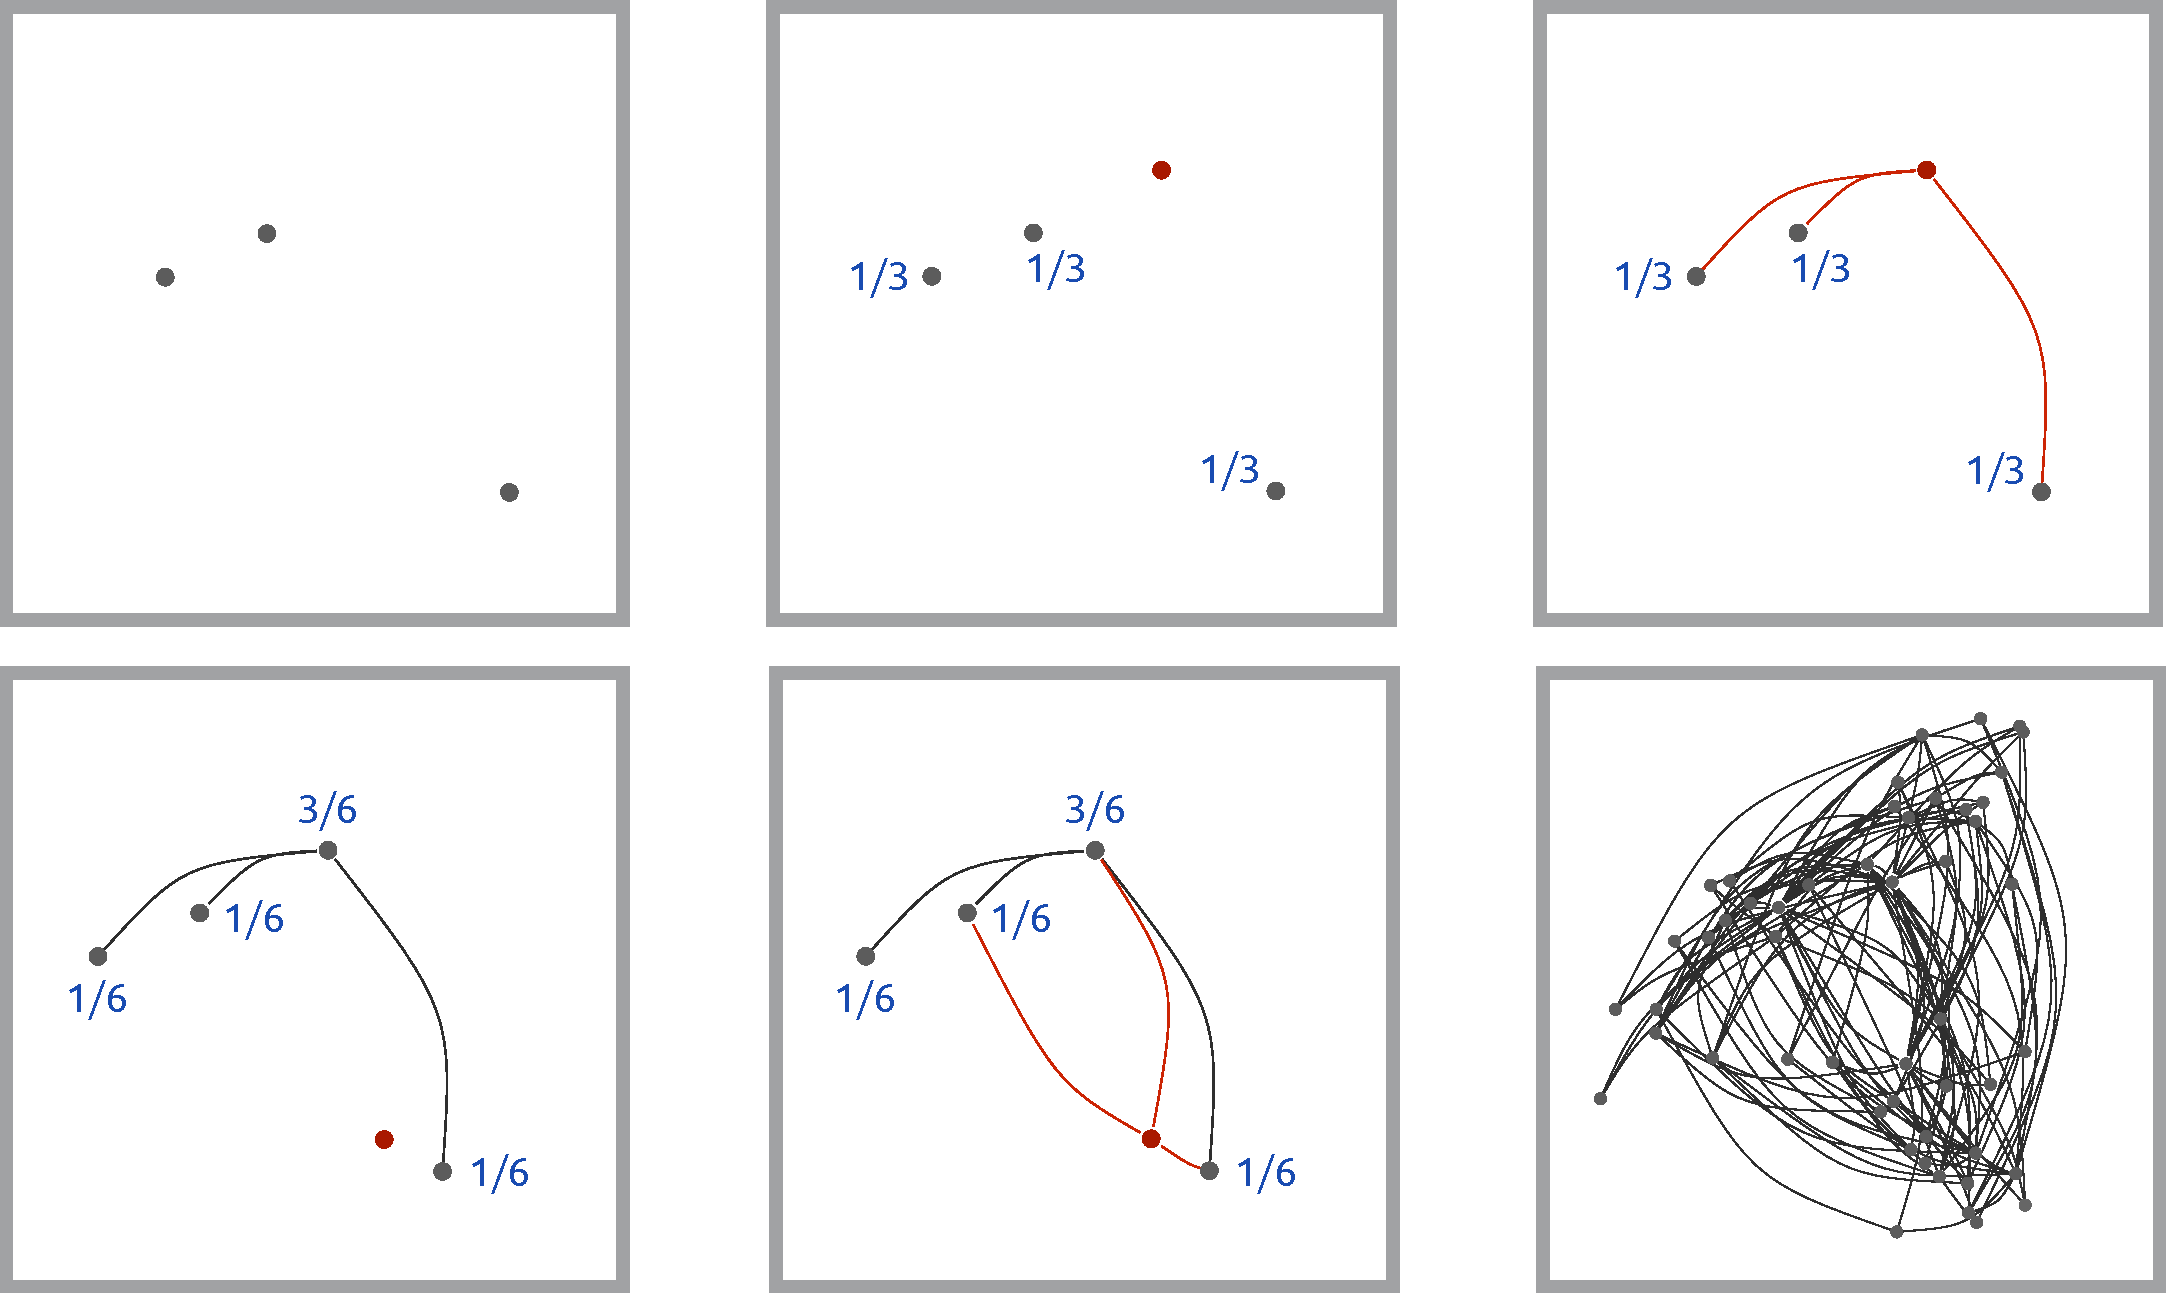
\includegraphics[width=0.9\textwidth]{pictures/21_begin.pdf}
    \marginnote{A.2.1}
    \caption{The first steps of the Barab\'asi-Albert algorithm with $m
    = m_0 = 3$. From left to right and from top to bottom single nodes are
    first added before edges are chosen according to the preferential
    attachment probabilities printed in blue. The last picture shows the network
    after 47 nodes have been added.}
    \label{fig:21_begin}
\end{figure}

\begin{figure}
    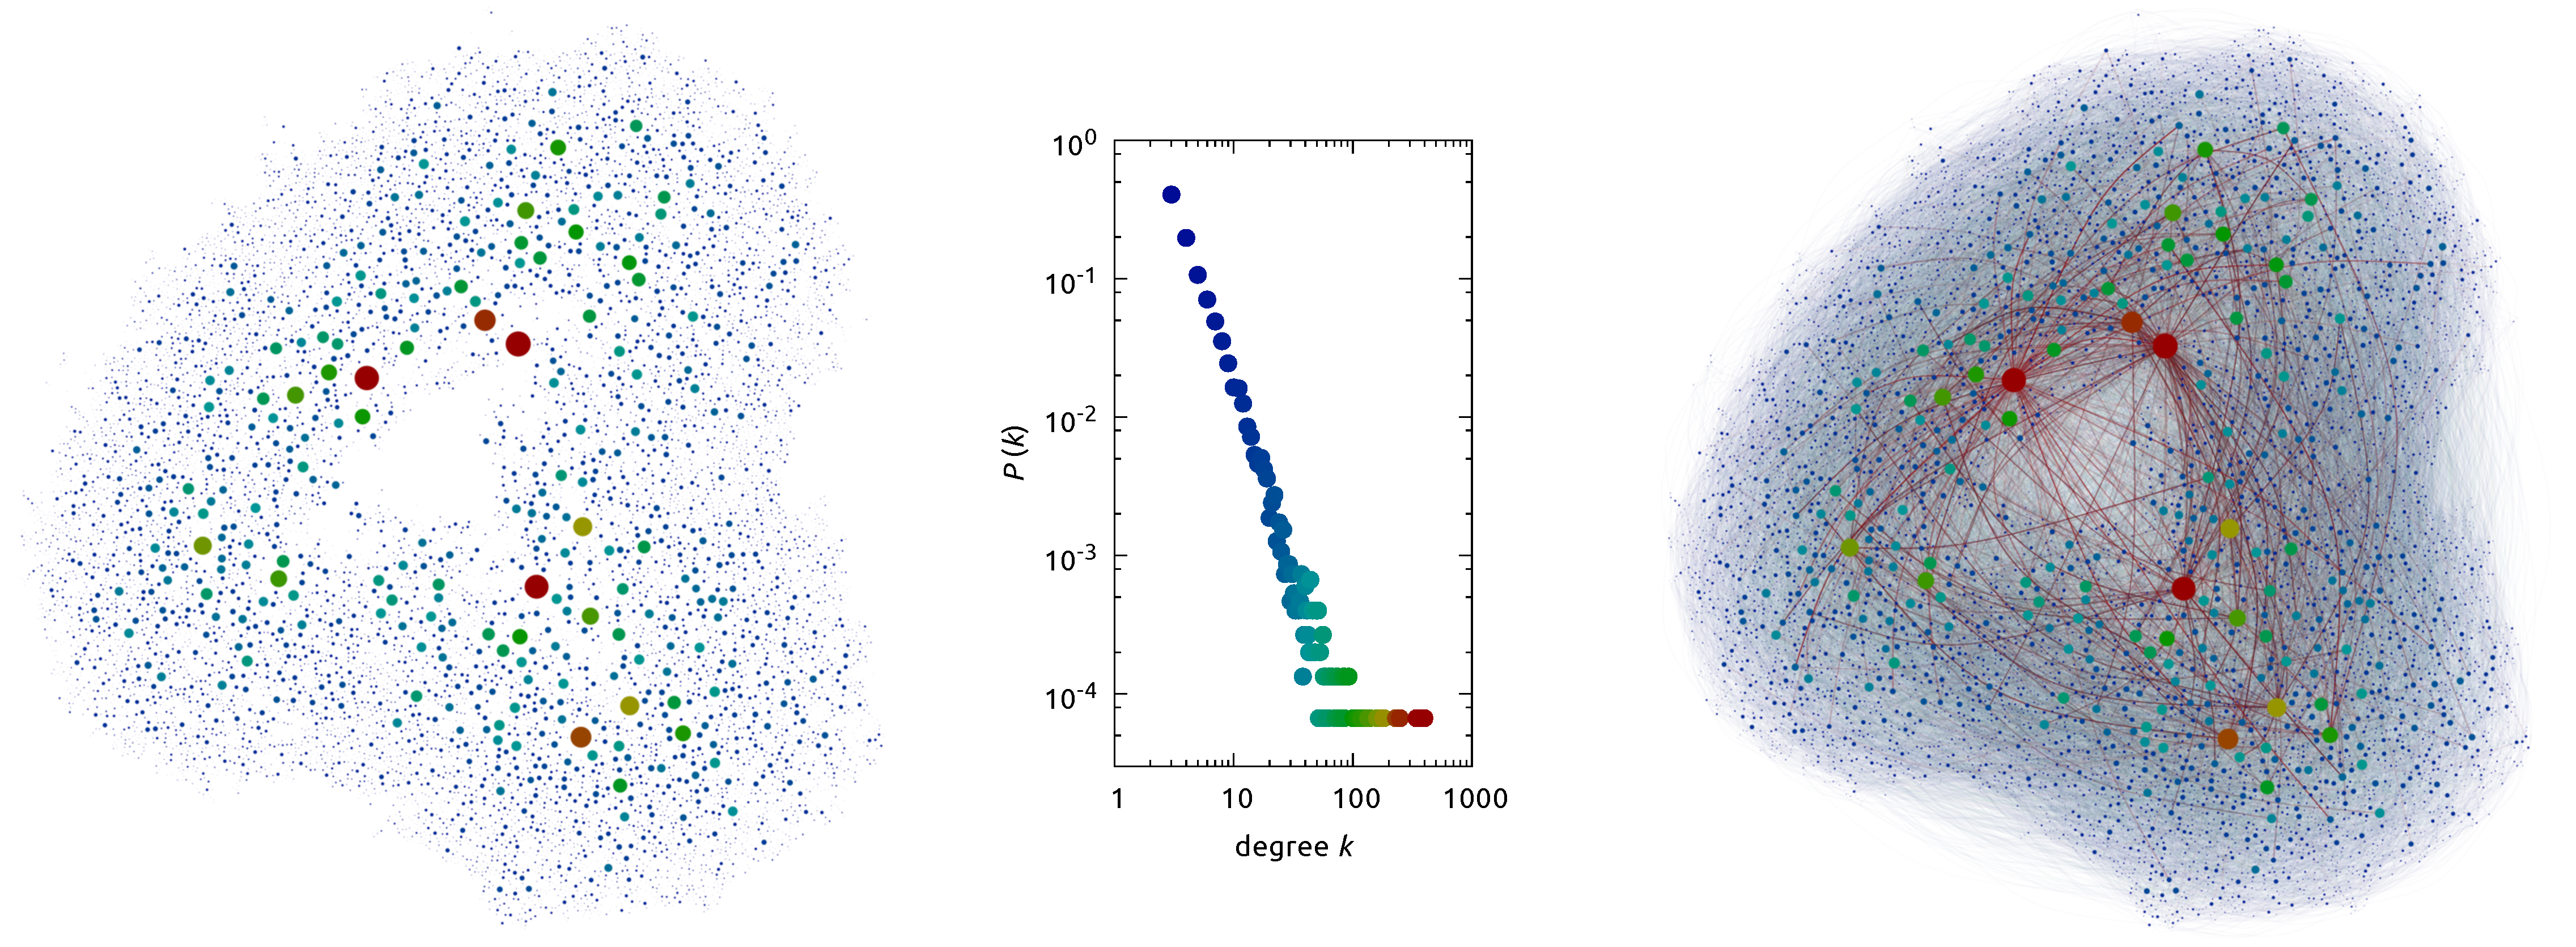
\includegraphics[width=\textwidth]{pictures/21_end.pdf}
    \marginnote{A.2.1 A.2.2}
    \caption{The same network as in figure \ref{fig:21_begin} after 15000
    nodes have been added (left: without drawing the edges, and right: with
    drawing the edges). The color and the size of the nodes printed in the left
    and right picture describe the degree of the respective node. The
    picture in the middle shows the degree distribution (with the same color
    keys as in the node coloring).}
    \label{fig:21_end}
\end{figure}

\begin{figure}
    \gnuplotloadfile[terminal=epslatex, terminaloptions={color size 6,3}]{pictures/22_plot.gp}
    \marginnote{A.2.2}
    \caption{Degree distribution for a simulation of a Barab\'asi-Albert
    network with $N=500000$ nodes in total, using different values for
    $m$. The line has a slope of $-3$.}
    \label{fig:22_plot}
\end{figure}
\begin{figure}
    \gnuplotloadfile[terminal=epslatex, terminaloptions={color size 6,3}]{pictures/22_logplot.gp}
    \marginnote{A.2.2}
    \caption{The same degree distribution as in figure \ref{fig:22_plot}
    using logarithmic binning so that the the points plotted are the average
    values over equidistant bins on the logarithmic axis (i.e. the bin width
    increases exponentially).}
    \label{fig:22_logplot}
\end{figure}

\begin{figure}
    \gnuplotloadfile[terminal=epslatex, terminaloptions={color size 6.2,4}]{pictures/24_ba.gp}
    \vspace*{-0.75cm}
    \marginnote{A.2.3 A.2.4 A.2.5}
    \caption{Numerical robustness analysis for Barab\'asi-Albert (BA) networks
    (as model for scale-free networks) and Erdös-Renyi (ER) networks under
    the influence of different strains (failure, hub attacks and
    \enquote{evil} attacks, described in the text). In each case, networks
    of the size $N=500$ were first created and then stepwisely disassembled
    by taking away nodes (and thus increasing $p_\mathrm{lost}$. The
    parameter for the Barab\'asi-Albert networks was $m = 4$ (??), while
    $p=0\cdots$ (??) was used for the Erdös-Renyi networks. The vertical
    lines stopping at the respective maximal values of the (finite) average
    cluster size $\langle s\rangle^\mathrm{f}$ can be used to read off
    estimates for the percolation thresholds $p_c$ of the respective
    processes. So if the $p_\mathrm{lost}$ value of such a vertical line is
    $p$, then the corresponding percolation threshold is $p_c = 1-p$.}
    \label{fig:24_ba}
\end{figure}

\clearpage
\clearpage


\section{Random Network Percolation}
The process of percolation appears in many systems of interest to physics
and network science in general. The main feature of networks (with a fixed
number $N$ of nodes) undergoing percolation is the (often sudden) emergence
of a single \emph{giant component} when the number of edges is increased.

The critical threshold value $p_c$ for the \emph{occupation probability}
(the fraction of present edges to all possible edges), for which the
probability that a giant component arises becomes non-zero, is usually
different for different networks. There are however some indicative
quantities for percolation whose scaling behavior depends only on the
\emph{dimension} of the network in question. In this context the dimension $d$
of a graph is the smallest natural number for which the graph can be embedded in
$\mathbb{Z}^d$ so that every edge only connects nodes with manhattan distance 1.
A special case are graphs with dimension $d=\infty$, which can not be embedded in any
$\mathbb{Z}^d$ meeting the above criterium.

Two important indicative quantities for percolation are the
\emph{percolation probability} $P$, which is the probability that a node
belongs to the \emph{giant component}, and the (finite) \emph{average
cluster size} $\langle s \rangle^\mathrm{f}$, which measures the average
cluster size of the finitely large components. According to percolation theory, one has
\begin{equation}\label{eq:coefficients}
\begin{aligned}
    P(p) \sim (p - p_c)^\beta \\
    \langle s \rangle^\mathrm{f}(p) \sim (p - p_c)^\gamma
\end{aligned}
\end{equation}
for suitable scaling exponents $\beta$ and $\gamma$ (that depend on the dimension only).


\subsection{Percolation in two and infinitely many dimensions}
\marginnote{A.3.1} Simulations that create percolation behavior for $d=2$
and $d=\infty$ were conducted in the following manner:
\begin{itemize}
    \item Create a network with $N$ nodes and the maximal number of edges
        for the respective dimension. For $d=2$ this simply was a completely
        connected two dimensional grid with $N = n^2$ nodes; for $d=\infty$
        this was a completely connected graph of size $N$.
    \item Now randomly select edges which are to be removed in every step.
    \item For every such step, several quantities were recorded: 
    \begin{itemize}
        \item The occupation probability $p = \frac{\text{current number of
            edges}}{\text{initial number of edges}}$.
        \item The sizes $\mathrm{max}_C$ and $\mathrm{max}_C^\mathrm{f}$ of the largest and
            second largest components. The $^\mathrm{f}$ stands for the
            maximal size over the \enquote{finite} clusters, meaning all
            but the largest.
        \item The average cluster size $\langle s\rangle$ and the finite 
            average cluster size $\langle s\rangle^\mathrm{f}$.
        \item The degree distribution $P_\mathrm{d}(k)$ and the cluster size distribution $P_C(k)$.
    \end{itemize}
\end{itemize}
The obtained results can be seen in figures \ref{fig:31_2d} and
\ref{fig:31_2d_dist} for $d=2$ as well as \ref{fig:31_infty} and
\ref{fig:31_infty_dist} for $d=\infty$.

\marginnote{A.3.2} Next, the data retrieved in the simulation described
previously was used to estimate the scaling exponents $\beta$ and $\gamma$
for $d=2$ as well as $d=\infty$. For this end, the formulas in
\eqref{eq:coefficients} were applied by conducting a linear regression of
$\log P$ respectively $\log \langle s\rangle^\mathrm{f}$ against
$\log(p-p_c)$.
There are two things one must pay attention to: First of all, the given
formulas only hold exactly in the limit of $N\to\infty$, so for a example
a real divergence expected for $\langle s\rangle^\mathrm{f}$ at $p_c$
cannot take place. This means, that the data will certainly deviate from
the power-law if too near to $p_c$. On the other hand however, the given
formulas only hold near $p_c$, so one must fix both a minimal value $m>0$
and a maximal value $M>0$ so that the points that enter the regression are
described by $m < p-p_c < M$. 

The corresponding log-log plots as well as the resulting fitting line
together with the choice of $m$ and $M$ for the four different situations
($\alpha$ and $\beta$ for both $d=2$ and $d=\infty$) are depicted in
figures \ref{fig:32_2d} and \ref{fig:32_infty}. For the simulation the
quantity $P$ was identified with the relative size of the largest component
and $\langle s\rangle^\mathrm{f}$ was taken to be the average cluster size
for all but the largest cluster. The obtained values $\beta$ and $\gamma$,
compared to the theoretical ones (denoted by $\beta_\mathrm{theo}$ and
$\gamma_\mathrm{theo}$, are as follows:

\begin{center}
    \begin{tabular}{r@{\qquad\qquad}c@{\quad}c@{\qquad\quad}c@{\quad}c}
    $d$ & $\beta$ & $\beta_\mathrm{theo}$ & $\gamma$ & $\gamma_\mathrm{theo}$ \\
    \hline
    $2$ & $0.288$ & $0.14$ & $-3.56$ & $-2.25$   \\
    $\infty$ & $0.718$ & $1$ & $-2.085$ & $-1$ \\
\end{tabular}
\end{center}

Comparing the produced and the predicted values, the results obtained
by simulation can only be regarded as a very rough estimate. Problems
leading to this are probably the low value of $N$, the arbitrariness when
deciding on $m$ and $M$, as well as the fact that e.g. for $d=\infty$ the used
value $p_c=1/N$ is only true for large $N$.


\subsection{Explosive Percolation}
Percolation processes in different systems possess different shapes -- the
transitions can be rather smooth or very sharp. Under certain
circumstances, the latter phenomenon is labeled \emph{explosive
percolation}. A common rule to generate explosive percolation
is the \emph{product rule}.

\marginnote{A.3.3} Firstly, simulations were conducted to compare the
percolation processes of the Erdös-Renyi rule of adding edges and the
product rule. To do so, empty networks with $N$ nodes were initialized and
successively filled with edges, according to the respective algorithm. At
every step the quantity $P$ (the relative size of the largest cluster, see
above) was determined and plotted (see figure \ref{fig:33_perc} a)). The
sharpness of the rise is then a (qualitative) measure for the
\enquote{explosiveness} of the percolation transition.

The obtained results show that the product rule indeed produces a more
explosive transition than the Erdos-Renyi rule.

\marginnote{A.3.4} Of course there are many other rules that produce
explosive percolation (partially even much sharper than the product rule)
and also rules that prevent the percolation from being explosive
altogether. In order to make this clear, two extreme cases, labeled
\enquote{extreme} and \enquote{anti-extreme}, have been introduced (see
next paragraph).  As a second example of non-explosive percolation (besides
the \enquote{anti-extreme} rule) an \enquote{anti-product} rule was
introduced, which simply switches the sign of the
\enquote{greater-or-equal} relation in the decision process to read
\enquote{smaller-or-equal}. The resulting percolation transitions for these
three models are visualized in figure \ref{fig:33_perc} b).

The \enquote{extreme} rule always connects nodes from \emph{different}
clusters of \emph{minimal} size. This makes sure that the largest component
stays small for quite some time but will then grow even faster than
exponentially. 
The \enquote{anti-extreme} rule also always connects nodes from different clusters,
but picks nodes from the clusters with \emph{maximal} size. This way the explosion process
is completely prevented and the growth of $P$ is linear.

\begin{figure}
    \gnuplotloadfile[terminal=epslatex, terminaloptions={color size 6.5,2.0}]{pictures/31_2d.gp}
    \marginnote{A.3.1}
    \caption{Several quantities plotted as function of the occupation probability
        $p$, describing the percolation process in two dimensions for
        $N=625$. Figure \textbf{a)} shows the size $\mathrm{max}_C$ of the
        largest cluster (which would be the infinite cluster for $N
        = \infty$) as well as the average cluster size $\langle s\rangle$.
        Figure \textbf{b)} contains the size $\mathrm{max}_C^\mathrm{f}$ of
        the second largest cluster (which would be the biggest
        \enquote{finite} cluster for $N=\infty$) and the average cluster
        size $\langle s\rangle^\mathrm{f}$ for all but the largest cluster.
        The results were averaged over 500 trials and the simulation was
        conducted backwardly by stepwisely removing random edges from a full
        2d graph. The grey line marks the percolation threshold $p_c=0.5$ for
        this simulation.}
    \label{fig:31_2d}
\end{figure}

\begin{figure}
    \gnuplotloadfile[terminal=epslatex, terminaloptions={color size 6.5,2.0}]{pictures/31_2d_dist.gp}
    \marginnote{A.3.1}
    \caption{Results for the degree distribution $P_\mathrm{d}(k)$ and the
        cluster size distribution $P_\mathrm{C}(s)$ for different
        values of the occupation probability $p$ for 2d percolation with
        a network size of $N=625$ (see also figure \ref{fig:31_2d}). Note that the
        lines connecting the dots (there are only discrete values for the
        probabilities) are meaningless and only included to make it easier to
        keep track of the distributions.}
    \label{fig:31_2d_dist}
\end{figure}

\begin{figure}
    \gnuplotloadfile[terminal=epslatex, terminaloptions={color size 6.5,2.0}]{pictures/31_infty.gp}
    \marginnote{A.3.1}
    \caption{The same quantities as presentend in figure \ref{fig:31_2d}
        for an infinite dimensional grid. This time, edges were successively
        removed from a fully connected graph with 250 nodes. Again, 500 trials were
        averaged. They grey line is drawn at $p=1/N=1/250=0.004$, which is the theoretic prediction
        of the percolation threshold for large $N$.}
        %Next to the grey line at $p=1/250=0.004$, which would be the theoretic prediction of the
        %percolation threshold for large $N$, the red line at $p\approx 0.0046$
        %marks the maximum of $\langle s \rangle^\mathrm{f}$. This second value works better
        %for $p_c$ than the theoretical prediction in this case,
        %probably because $N$ is too small.}
    \label{fig:31_infty}
\end{figure}

\begin{figure}
    \gnuplotloadfile[terminal=epslatex, terminaloptions={color size 6.5,2.0}]{pictures/31_infty_dist.gp}
    \marginnote{A.3.1}
    \caption{The degree distribution (\textbf{a)}) and cluster size
        distribution (\textbf{b)}) for different values of $p$ for infinite
        dimensional percolation. The data were collected in the simulation
        described in figure \ref{fig:31_infty}.}
    \label{fig:31_infty_dist}
\end{figure}

\begin{figure}
    \gnuplotloadfile[terminal=epslatex, terminaloptions={color size 6.5,2.0}]{pictures/32_2d.gp}
    \marginnote{A.3.2}
    \caption{Log-log plots of \textbf{a)} the largest cluster's size
        $\mathrm{max}_C$ and \textbf{b)} the average finite cluster size
        $\langle s\rangle^\mathrm{f}$ as function of $p-p_c$ for 2d
        percolation, where $p_c=0.5$. The grey area marks the points that were
        used for the linear regression in order to find the percolation
        coefficients.}
    \label{fig:32_2d}
\end{figure}

\begin{figure}
    \gnuplotloadfile[terminal=epslatex, terminaloptions={color size 6.5,2.0}]{pictures/32_infty.gp}
    \marginnote{A.3.2}
    \caption{Log-log plots of \textbf{a)} the largest cluster's size
        $\mathrm{max}_C$ and \textbf{b)} the average finite cluster size
        $\langle s\rangle^\mathrm{f}$ as function of $p-p_c$ for infinite dimensional
        percolation, where $p_c=0.004$ is the theoretic prediction of the
        percolation threshold. The grey area marks the points used for the linear
        regression in order to find the percolation exponents. Using other
        values of $p_c$, for example the maximum of $\langle
        s\rangle^\mathrm{f}$ (see figure \ref{fig:31_infty} b)) did not yield
        more linear graphs or better coefficients.}
    \label{fig:32_infty}
\end{figure}

\begin{figure}
    \gnuplotloadfile[terminal=epslatex, terminaloptions={color size 6.5,2.0}]{pictures/33_perc.gp}
    \marginnote{A.3.3 A.3.4}
    \caption{Percolation transitions for different rules for adding edges,
        starting with an empty network of $n=500$ nodes. Figure \textbf{a)}
        compares the Erdös-Renyi and the product rule, whereas figure
        \textbf{b)} shows the transitions for three other rules that either create
        smoother transitions than the Erdös-Renyi and product rule
        (anti-product and anti-extreme rule) or create an even much sharper
        transition (extreme rule). }
        %The \textbf{\enquote{anti-product} rule} simply changes the
        %'less-or-equal' relation of the product rule in
        %a 'greater-or-equal' relation. The \textbf{\enquote{extreme} rule}
        %systematically connects the two smallest existing components in every
        %step, which causes an extremely explosive transition. The \textbf{\enquote{anti-extreme} rule}
        %systematically connects the two largest components in every step, which makes the growth
        %linear and thus strongly unexplosive.}
    \label{fig:33_perc}
\end{figure}


\end{document}
